\label{ch:eda-chapter}

The following chapter proposes a dissertation on the merits of the previously mentioned \textbf{Electrodermal Activity} and its potential implications in the context of fall detection.

% TODO maybe change title
\section{Key Aspects of Skin Conductance Analysis}\label{sec:eda-description}

In the whole field of bio-signals, a subject of interest in the recent years has been the so-called \textbf{Electrodermal Activity}, also known as \textbf{Skin Conductance} or \textbf{Galvanic Skin Response}.

The latter describes the continuous variations of the electrical conductivity of the skin (which is also referred as Skin Conductance or SC) and has been depicted as the main criteria to investigate the psychophysiological states of an individual since the beginning of the 20th century.

\subsection{EDA signals and correlation with psychophysiological stress detection}\label{subsec:eda-signals}

As stated in section \ref{sec:edaintro}, the Electrodermal Activity provides a non-invasive technique to analyze the activity of the \textbf{autonomic nervous system} (ANS) by measuring the resistance opposed by the skin to the electrical current, which varies according to the \textbf{sweat glands} activity.

Perspiration is, in fact, governed by the sympathetic nervous system \cite{bartholomew} through the postganglionic sudomotor fibers, in connection with the external stimulations received. On these principles, a situation of emotional distress that induces an excitement of the ANS activity would also cause changes in sweat secretion. The measuring of the latter may, then, provide a qualitative indicator related to the \textbf{emotional response} of a subject \cite{carlson}.

\begin{figure}[h]
    \centering
    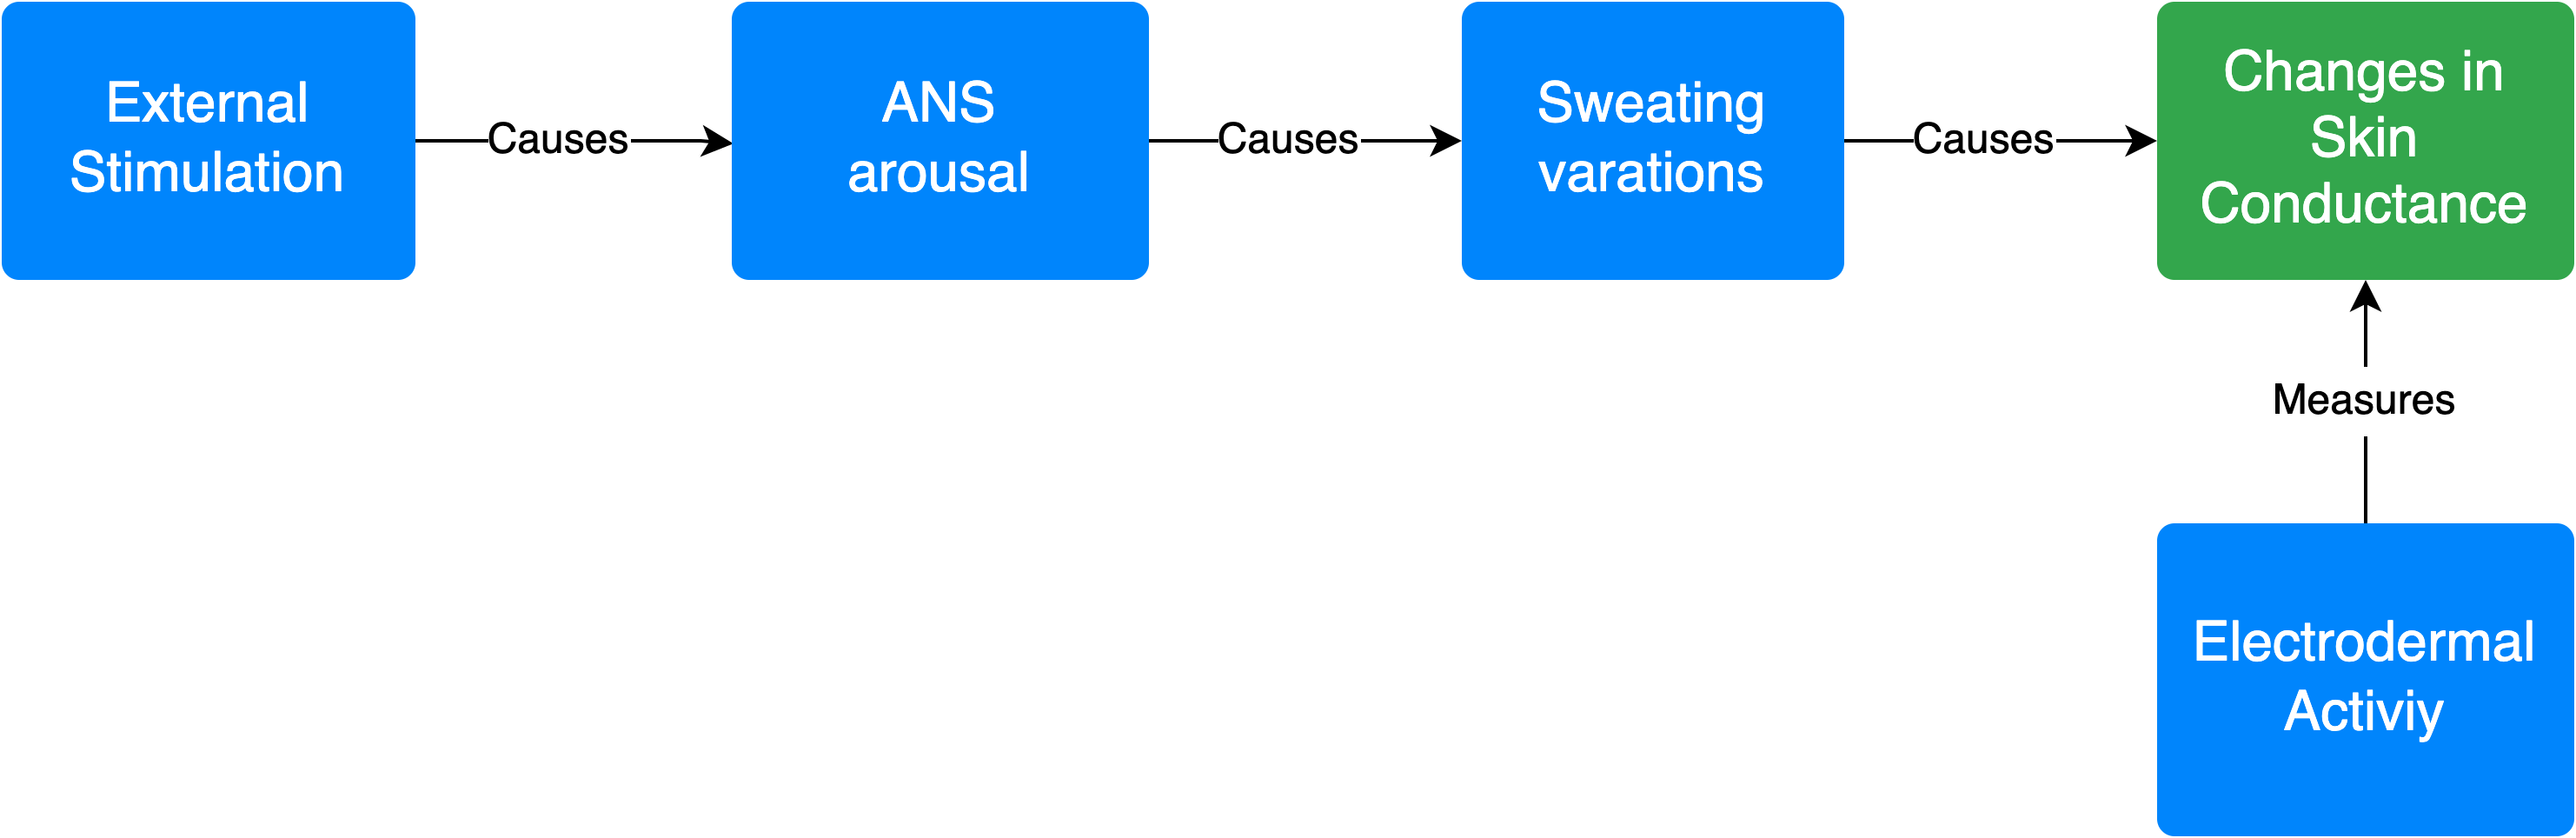
\includegraphics[width=\textwidth]{./images/eda-cause-effect.drawio.png}
    \caption{Correlation between Electrodermal Activity and the Autonomic Nervous System}
    \label{fig:eda-ans}
\end{figure}

\subsection{Measurement}\label{subsec:eda-measurement}

% https://www.birmingham.ac.uk/Documents/college-les/psych/saal/guide-electrodermal-activity.pdf

In order to detect Electrodermal Activity on and individual's skin, two different approaches may be employed:

\begin{itemize}
    \item Exosomatic Methodology
    \item Endosomatic Methodology
\end{itemize}

The first one tends to be the most commonly used and implies the application of a direct or alternating current directly on the skin. The second one, instead, does not involve the usage of any external current.

% https://www.tobiipro.com/learn-and-support/learn/GSR-essentials/how-does-a-gsr-sensor-work/
The implementation of the exosomatic methodology requires the usage of \textbf{two electrodes} through which a voltage of direct current of 0.5 VDC is trasmitted. After being applied to the skin, the current flow through the electrodes is measured by applying the \textbf{Ohm's Law}, which determines the resistance opposed by the epidermis.

\begin{figure}[h]
    \begin{equation}
    \begin{aligned}
    I = \frac{U}{R} \\
    \\
    R = \frac{U}{I}
    \end{aligned}
    \end{equation}
    \caption{Ohm's Law Formula}
    \label{fig:ohmlaw}
\end{figure}

It is important to place both the electrodes on the palm of the hand, on two adjacent fingers or, otherwise, on the sole of the foot. These areas have been, in fact, identified as the most prominent in terms of perspiration. Modern EDA sensors employ electrodes with Ag/AgCl contact points in order to accurately transmit the electrical current \cite{eda-imotions}. Isotonic gel is also generally used to accommodate the signal transmission from the skin and consequently improve its quality.

\begin{figure}[h]
    \centering
    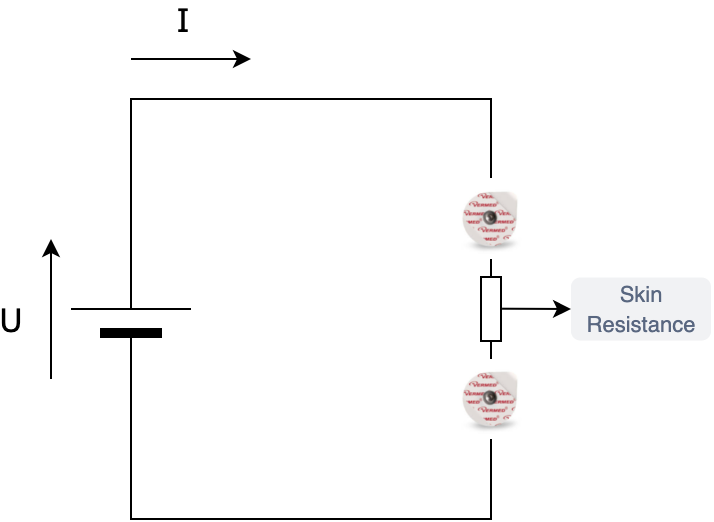
\includegraphics[width=8cm]{./images/skin-resistance.drawio.png}
    \caption{Representation of the EDA measurement principle}
    \label{fig:eda-ans}
\end{figure}

The resistance obtained is expressed in terms of the \textbf{Siemens} ($S$) measuring unit. More specifically, because of the small values obtained, microSiemens ($\mu S$) are normally employed.

\subsection{Sample rates}\label{subsec:eda-signal-properties}

EDA is regarded as a slow measure \cite{eda-guide}. According to the related literature, typical frequency intervals are, in fact:

\begin{itemize}
    \item 0 - 3 Hz \cite{biosignalplux-guide}
    \item 0 - 10 Hz \cite{eda-hci}
    \item 0.0167 - 0.25 Hz \cite{eda-interval-3}
    \item 0.045 - 0.25 Hz \cite{eda-interval-4}
    \item 0.05 - 35 Hz \cite{eda-guide}
\end{itemize}

By applying the \textbf{Nyquist Theorem} \cite{nyquist}, which states that a signal should be sampled at least at two times its highest frequency, it can be inferred that EDA signals must be sampled at 70 Hz or more. In practice, sample rates between 70 Hz and 400 Hz are commonly used according to the requirements of the experimentation in order to provide greater accuracy during the signal processing stage \cite{eda-guide}. Lowpass and bandpass filters are, then, applied in order to smooth the signal and remove unwanted \textbf{noises}.

\subsection{Phasic and Tonic component}\label{subsec:phasic-tonic}

EDA signals are characterized by two \textbf{additive} components \cite{eda-guide} referred as:

\begin{itemize}
    \item \textbf{Tonic component} (also known as Skin Conductance Level or SCL)
    \item \textbf{Phasic component} (also known as Skin Conductance Response or SCR)
\end{itemize}

While the tonic component describes the slowly and continuously changing part of the signal, the phasic component depicts, instead, a fast changing signal whose variations are determined by event-related stimulations.

In order to decompose the measurement obtained in its components, an approach based on \textbf{standard deconvolution} can be employed. Assumed the additivity of the two signals, the skin conductance can be represented as follows:

\begin{equation}
    SC = SC_{tonic} + SC_{phasic}
\end{equation}

Furthermore, both the $SC_{tonic}$ and $SC_{phasic}$ components can be represented by a convolution operation which foresees the multiplication of a so-called \textbf{driver component} recorded by the sensor with an Impulse Response function \cite{edasvm}:

\vspace{5mm}

\begin{figure}[h]
\begin{equation}
SC = Driver_{tonic} \cdot IRF + Driver_{phasic} \cdot IRF
\end{equation}
\caption{Convolution process of the tonic and phasic components}
\label{fig:eda-convolution}
\end{figure}

In order to detect variations of an individual's arousal over a specific time interval, the phasic component obtained by the deconvolution process is generally employed for feature extraction purposes.

The example reported in Figure \ref{fig:eda-example} illustrates:

\begin{itemize}
    \item A raw EDA signal with a duration of 15 seconds depicting an increase in the arousal level
    \item The subsequently extrapolated SCR component
    \item The SCL component
\end{itemize}

\begin{figure}[h]
    \centering
    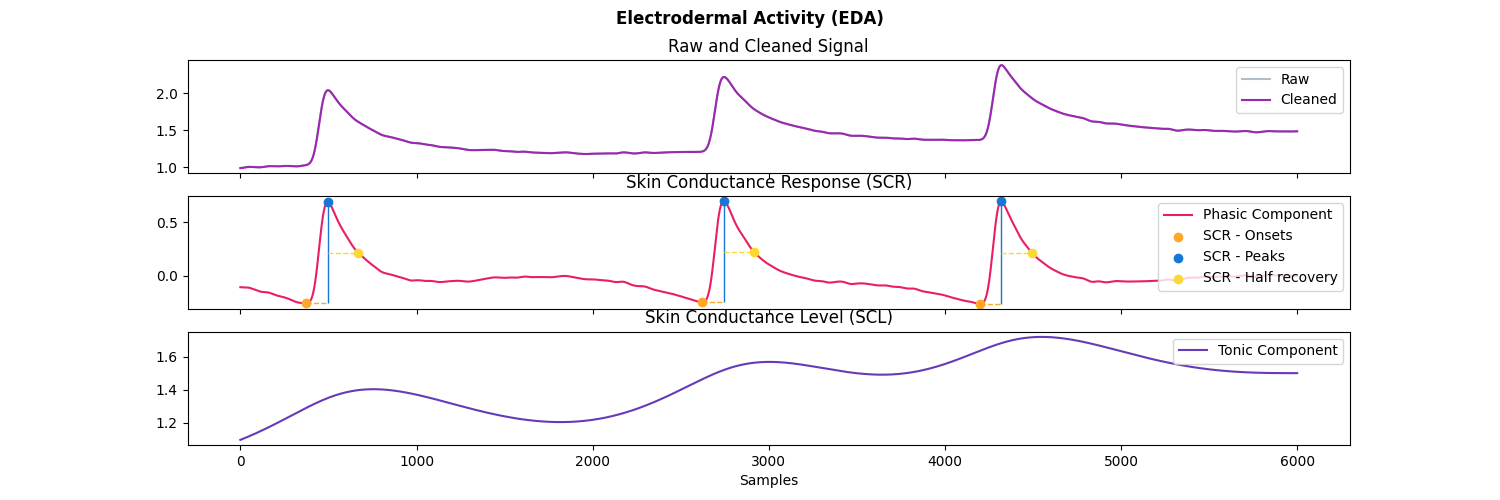
\includegraphics[width=\textwidth]{./images/eda-simulation.png}
    \caption{Decomposition of Raw EDA signal in its two components}
    \label{fig:eda-example}
\end{figure}

The raw signals were generated thorugh NeuroKit2, a Python Toolbox for Neurophysiological Signal Processing that implements several biosignal processing routines, including EDA-related ones \cite{neurokit}.

\subsection{Use Cases}\label{subsec:eda-usecases}

The application of psychophysiological sensors is becoming an increasingly frequent practice in the context of Human Computer Interaction \cite{eda-hci}. More specifically, the Electrodermal Activity may provide a measure to define the level of \textbf{arousal} that characterizes and individual during experimentations and, generally, the usage of specific technologies.

Recent studies involved, for example, the measurement of Heart Rate and Electrodermal Activity in order to define an objective evaluation method for experiences based on \textbf{virtual reality}. Moreover, excellent results have been obtained by Sánchez-Reolid \textit{et al., 2018}~\cite{edasvm}, whose classification model based on \textbf{Deep Support Vector Machines} achieved excellent results in the identification of stress patterns by employing EDA measurements acquired from a wearable device.

\section{Electrodermal Activity and Fall Detection Systems}\label{sec:eda-fall-detection}

The Electrodermal Activity measurement in the context of fall detection has not been a true object of interest yet. It is, however, reasonable to assume that analyzing the skin conductance response may help to provide additional information in order to help classifiers to reach higher levels of accuracy. 

In 2013, T. Horta \textit{et al., 2018}~\cite{eda-fall-detection} included EDA signals in the development of a system for fall detection and prevention based on biofeedback monitoring solutions. The latter obtained valid results, but the analysis performed by the authors did not aim to provide assessments on the influence that Electrodermal Activity had on the accuracy of the whole system (which include other bio-sensors such as electroencephalography, electrocardiogram, electromyography and blood volume pressure).

\subsection{Correlations between EDA and Wearable Devices}\label{subsec:eda-wearables}

Because of the nature of EDA signals, during the years the main object of interest has been monitoring patients over extended periods of time and in real-life situations in order to identify patterns that are difficult to replicate in artificial environments. This has consequently focused the interest of researchers in the development of wearable devices for the electrodermal activity measurement \cite{poh-wearable}. 

In 2010, Poh \textit{et al., 2018}~\cite{poh-wearable} described one of the first implementations of a compact and cost-effective wearable sensor for unobtrusive and long-term assessment of Electrodermal Activity. This was packed inside a wristband exposing two electrodes. The outcomes obtained were strongly correlated with FDA-approved measurement systems. Furthermore, over the last decade several companies such \textbf{Empatica} (an MIT spin-off) or \textbf{Movisens GmbH} (a global leader in ambulatory assessment solutions) implemented highly performing wearable devices for EDA measurement which have been commonly employed in the field of research.

Additionally, at the end of September 2020 \textbf{Fitbit} released \textbf{Sense}, the first commercial wearable device implementing EDA measurement as one of its key features \cite{fitbit-eda}. This opened the way to new opportunities for developers, that will ghopefully be able to build software in order to measure and analyse the Electrodermal Activity by employing Application Programming Interfaces of commercial and commonly diffused devices, without having to rely on expensive and invasive equipment.

% Useful? 

% https://www.ncbi.nlm.nih.gov/pmc/articles/PMC2892750/#:~:text=Electrodermal%20activity%20(EDA)%20refers%20to,et%20al.%2C%201981).


